\documentclass[12pt]{article}
%Gummi|065|=)
\usepackage{amsmath, amsfonts, amssymb}
\usepackage[margin=0.5in]{geometry}
\usepackage{xcolor}
\usepackage{graphicx}

\newcommand{\off}[1]{}
\DeclareMathSizes{20}{30}{20}{18}

\newcommand{\two }{\sqrt[3]{2}}
\newcommand{\four}{\sqrt[3]{4}}
\newcommand{\red}{\begin{tikz}[scale=0.25]
\draw[fill=red, color=red] (0,0)--(1,0)--(1,1)--(0,1)--cycle;\end{tikz}}
\newcommand{\blue}{\begin{tikz}[scale=0.25]
\draw[fill=blue, color=blue] (0,0)--(1,0)--(1,1)--(0,1)--cycle;\end{tikz}}
\newcommand{\green}{\begin{tikz}[scale=0.25]
\draw[fill=green, color=green] (0,0)--(1,0)--(1,1)--(0,1)--cycle;\end{tikz}}

\usepackage{tikz}

\title{Nilsequences}
\author{John D Mangual}
\date{}
\begin{document}

\fontfamily{qag}\selectfont \fontsize{12.5}{15}\selectfont

\maketitle

\noindent Last month's sketch totally went nowhere. We will try to find sequences $a: \mathbb{N} \to \mathbb{C}$ or sets of integers $A \subseteq \mathbb{Z}$ and .  There seems to be an emerging theory for second order nilsequences (``quadratic fourier analysis") but not for higher nilsequences.  Like a good librarian I have collected as many resources as I can find -- some people have figured out different aspects about what these nilspaces look like. \\ \\
I will post this now and hopefully I can find something to say in two weeks!  
 
\vfill


\noindent 

\begin{thebibliography}{}

\item W.T. Gowers, Julia Wolf.  \textbf{Linear forms and quadratic uniformity for functions on $\mathbb{F}_p^n$} \texttt{1002.2209}

\item Ben Green, Terence Tao \textbf{Yet another proof of Szemeredi's theorem} \texttt{arXiv:1002.2254}

\item Balazs Szegedy \textbf{On higher order Fourier analysis} \texttt{arXiv:1203.2260}

\item Ben Green \textbf{Approximate algebraic structure} \texttt{arXiv:1404.0093}

\item Yonatan Gutman, Freddie Manners, P\'{e}ter P. Varj\'{u} \textbf{The structure theory of Nilspaces I} \texttt{arXiv:1605.08945}

\item W. T. Gowers \textbf{Generalizations of Fourier analysis, and how to apply them} \texttt{arXiv:1608.04127}

\item Ben Green, Terence Tao \textbf{New bounds for Szemer\'{e}di's theorem, III: A polylogarithmic bound for $r_4(N)$} \texttt{arXiv:1705.02080}

\item Freddie Manners \textbf{Good bounds in certain systems of true complexity 1} \texttt{arXiv:1705.06801}


\end{thebibliography}

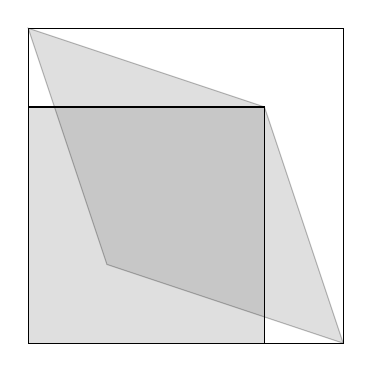
\begin{tikzpicture}
\draw (0,0)--(4,0)--(4,4)--(0,4)--cycle;
\draw[opacity=0.25, fill=black!50!white] (0,0)--(3,0)--(3,3)--(0,3)--cycle;
\draw (0,0)--(3,0)--(3,3)--(0,3)--cycle;
\draw[opacity=0.25, fill=black!50!white] (1,1)--(4,0)--(3,3)--(0,4)--cycle;
\draw (0,0)--(3,0)--(3,3)--(0,3)--cycle;
\end{tikzpicture}

\end{document}